\documentclass[11pt]{article}
\usepackage[a4paper,left=0.75in,right=0.75in,top=0.7in,bottom=0.75in]{geometry}
\usepackage{microtype}
\usepackage{graphicx,booktabs,tabularx,array,xcolor,enumitem,titlesec,amsmath}
\usepackage[unicode,hidelinks]{hyperref}
\definecolor{labgreen}{HTML}{204D32}
\definecolor{muted}{HTML}{56645B}
\definecolor{rulegreen}{HTML}{A8BEAC}
\hypersetup{pdftitle={PhotonicsAI Lab - Homework 4: Agentic Cell Erasing},pdfauthor={Aren Ananyan; David Sargsyan; Andranik Arakelyan; Yerem Bareghamyan},pdfsubject={From Prototype to Product: implementation, evidence, limitations and future applications}}
\pagestyle{plain}
\setlength{\parindent}{0pt}\setlength{\parskip}{5pt}
\setlength{\emergencystretch}{2em}
\setlist[itemize]{nosep,leftmargin=15pt,topsep=3pt}
\setlist[enumerate]{nosep,leftmargin=17pt,topsep=3pt}
\titleformat{\section}{\large\bfseries}{\thesection}{.6em}{}
\titleformat{\subsection}{\normalsize\bfseries}{}{0em}{}
\titlespacing*{\section}{0pt}{10pt}{5pt}
\titlespacing*{\subsection}{0pt}{7pt}{3pt}
\newcolumntype{Y}{>{\raggedright\arraybackslash}X}
\newcommand{\repo}{https://github.com/Arenananyan/PhotonicsAI-Lab-Cell-Erasing}
\newcommand{\smallcaption}[1]{{\small#1\par}}
\begin{document}
\begin{center}
{\small\textsc{PhotonicsAI}\quad |\quad\textsc{AI-Driven Science and Autonomous Laboratories}}\\[7pt]
{\Large\bfseries Homework 4}\\[4pt]
{\small From Prototype to Product: Agentic Cell Erasing}\\[5pt]
Aren Ananyan\quad |\quad David Sargsyan\\[3pt]
Andranik Arakelyan\quad |\quad Yerem Bareghamyan\\[5pt]
October 2026
\end{center}
\vspace{2pt}\hrule\vspace{5pt}
\textbf{Code, presentation and recordings:}\\
\href{\repo}{github.com/Arenananyan/PhotonicsAI-Lab-Cell-Erasing}

\section*{Task 1. Extend and demonstrate the hardware-integrated AI system}
\subsection{(a) Project objective and implemented extension}
We developed a prototype that connects natural-language requests to calibrated
visual measurements and supervised printer motion. A user can inspect colored
marks, select a cell by size or spatial relationship, review a path and authorize
one bounded operation. In this project, ``cells'' are blue and green marks on a
paper board; they are not biological cells.

The Homework 4 extension packages the hardware-facing components as a browser
product: a persistent conversation workspace, measured cell reports, board and
cell images, task suggestions, structured relational requests, operator approval,
and a queue for multiple targets. The emphasis is on turning separate device
interfaces into an inspectable, usable workflow.

\subsection{(b) System architecture}
\begin{tabularx}{\linewidth}{@{}p{32mm}Y@{}}
\toprule
\textbf{Component} & \textbf{Responsibility}\\\midrule
Browser frontend & Armenian/English conversations, history and deletion, light/dark themes, mobile layout, images, clarification and path approval.\\
Python backend & Task state, measured selection, conditions, scope validation, bounded execution and evidence records.\\
Groq model roles & Structured task interpretation, measured-ID selection, suggestions and visual assessment. The model proposes; the host validates.\\
Scanner MCP & Camera acquisition, board calibration, color detection, XY coordinates, areas and saved-frame artifacts.\\
Printer MCP & Status queries, complete-path preview, single-use execution tokens and constrained SSH/Klipper dispatch.\\
\bottomrule
\end{tabularx}

\subsection{The reusable interaction loop}
\textbf{Request $\rightarrow$ observe $\rightarrow$ measure/select $\rightarrow$
preview $\rightarrow$ human approval $\rightarrow$ execute $\rightarrow$ verify.}

The printer and scanner use separate MCP clients. Android IP Webcam supplies a
local image endpoint; an optional Blackmagic iPhone adapter provides camera
controls and preview. Tool evidence is treated as data, not as instructions.
Physical action remains separate from a model's interpretation of the request.

\newpage
\section*{(c) Reasoning, measurement and operator control}
\subsection{Implemented command families}
\begin{tabularx}{\linewidth}{@{}p{36mm}Y@{}}
\toprule
\textbf{Request} & \textbf{Resulting behavior}\\\midrule
Inspect or count & Read-only report of available measurements; blue and green cells are ranked separately.\\
Largest / smallest & Host checks the requested measured rank. Near-equal sizes within 5\% prompt a numbered choice with available cell crops.\\
Spatial relation & Find the blue cell nearest to the largest green cell, or report the distance between two size-selected cells.\\
If / then & Evaluate one supported count/area comparison on fresh calibrated evidence. A false condition finishes without motion.\\
Clean all & Freeze the initial eligible target queue, validate its paths, request one batch approval and attempt each target once.\\
Conversation reference & A previous selected cell can be referenced in the same chat; current geometry is re-observed before preparing a move.\\
\bottomrule
\end{tabularx}

\subsection{Geometry is calculated by the host}
For two calibrated cell centers, the reported distance is
\[
 d_{XY}=\sqrt{(x_2-x_1)^2+(y_2-y_1)^2}\quad\text{in millimeters.}
\]
The LLM receives measured IDs and geometry; it does not invent XY coordinates or
calculate the authoritative distance. Nearest candidates within 3 mm of each
other in distance require clarification. The 3 mm association tolerance is an
operating threshold, not a demonstrated positioning-accuracy guarantee.

\subsection{Fixed motion contract}
The configured observation HOME is $(209,208,100)$ mm, distinct from firmware
homing. The standard wipe uses an approach at $Z=100$ mm, configured contact
height $Z=14.5$ mm, a $Y+10$ mm offset and one clockwise circle of radius 10 mm,
then raises and returns HOME. Default speed is 20 mm/s; accepted task speeds are
bounded to at most 30 mm/s and further constrained by verified firmware limits.
These settings describe this setup and do not establish physical clearance.

\begin{itemize}
\item Fresh calibrated observations must stabilize before a target is accepted;
association is checked again before dispatch.
\item Complete paths, homing state, mesh/coordinate agreement, firmware bounds,
start position and motion gates are validated. The operator reviews clearance.
\item Preview tokens are short-lived and single-use. A transport failure with an
uncertain movement outcome never triggers an automatic motion retry.
\item Batch cleaning attempts each initial target once. Valid evidence of residue
is reported; an unavailable assessor can produce an uncertain result without
repeating that cell. Unusable camera evidence still pauses the workflow.
\end{itemize}

\subsection{Image-based result assessment}
The verifier compares the same target region before and after a wipe, including
colored-area measurements and an image-model assessment. More than 10\% measured
remaining color prevents a ``clean'' result. The possible verdicts are
\textit{clean}, \textit{residue} and \textit{uncertain}; they are visual assessments,
not proof of mechanical contact. Simulated movement is identified explicitly.

\newpage
\section*{(d) Product interface}
The website keeps successive requests in one conversation. New chats are explicit;
history, deletion, clarification and approval share the same workspace. Suggested
actions fill a draft rather than executing a tool. Board pictures and individual
cell crops are tied to their captured frame.

\begin{center}
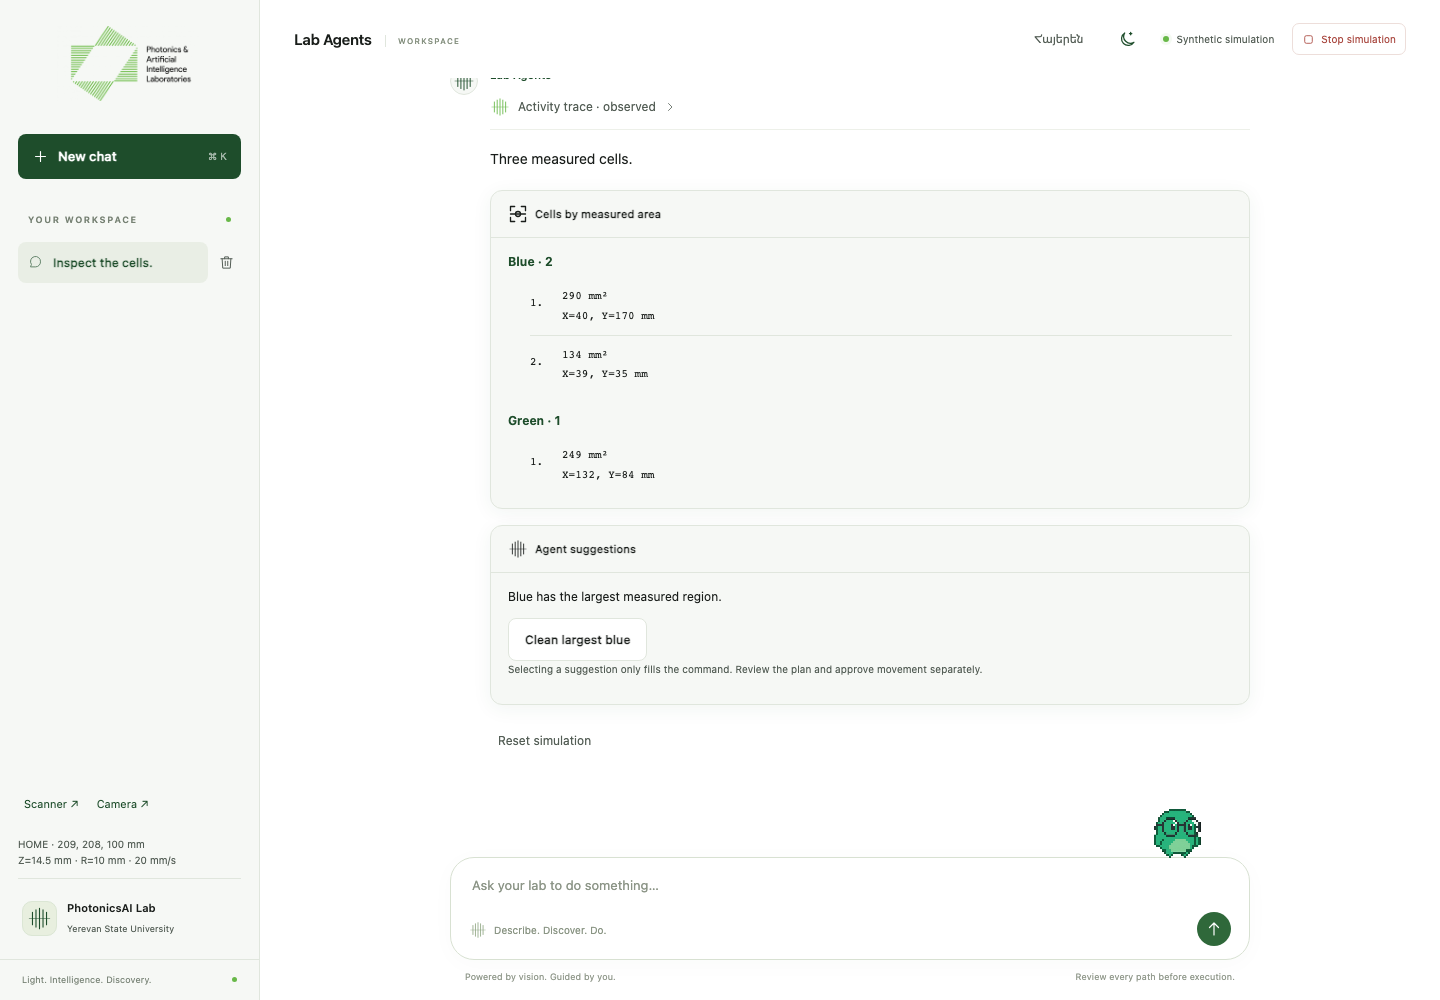
\includegraphics[width=.94\linewidth,height=84mm,keepaspectratio]{../../screenshots/01-desktop-light.png}
\end{center}
\smallcaption{Figure 1. Desktop workspace in the light theme. This screenshot is from an offline UI test with simulated API data; it is not a live hardware result.}

\begin{center}
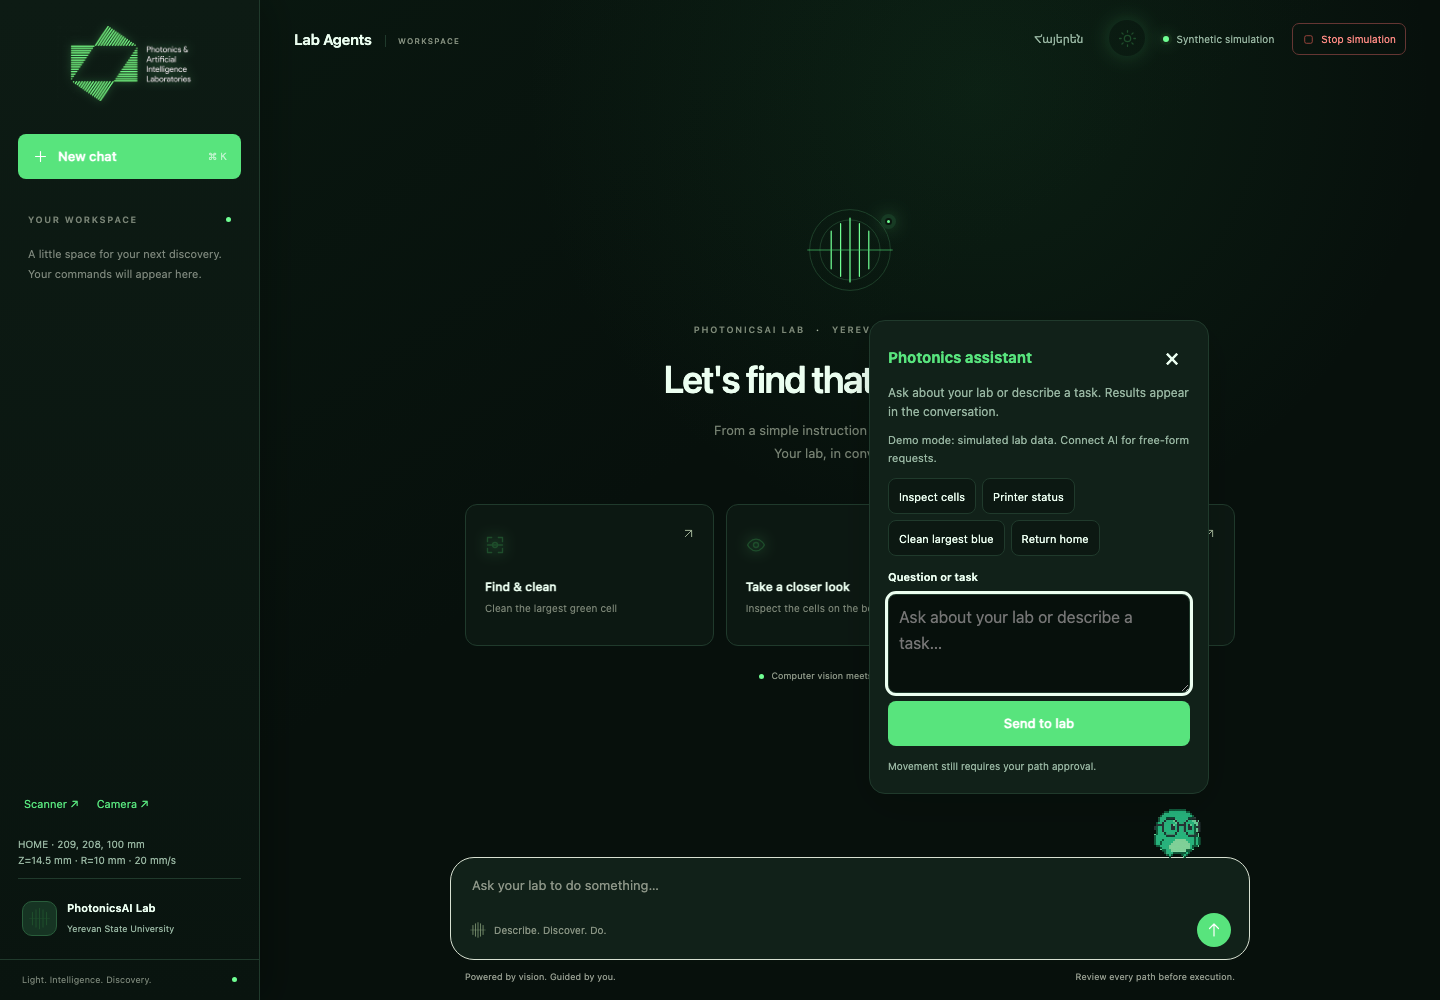
\includegraphics[width=.94\linewidth,height=84mm,keepaspectratio]{../../screenshots/02-desktop-dark-assistant.png}
\end{center}
\smallcaption{Figure 2. Dark theme and assistant panel. The panel enters the same conversation workflow; shortcuts do not bypass motion approval. Offline UI-test screenshot.}

\subsection{Local deployment and remote access}
The application runs locally; a phone on the same network can access the dashboard
when it is bound to the network interface. Remote browsers require the generated
local login. The current HTTP deployment is intended for a trusted lab network;
a production deployment would require stronger transport and access controls.
Camera-specific calibration must be performed for the actual setup.

\newpage
\section*{(e) Validation and supplied evidence}
The submission copy was checked with the existing local Python environments.
All listed software checks passed. Test fixtures, local sockets and mocked APIs
were used; no real motion or live Groq request was issued during packaging.
\begin{center}
\begin{tabularx}{\linewidth}{@{}Yrp{73mm}@{}}
\toprule
\textbf{Suite} & \textbf{Passed} & \textbf{Scope}\\\midrule
Printer & 143 & Policy, mock state, local sockets, schemas and MCP\\
Scanner & 61 & Synthetic images, calibration, detection and camera-source API\\
Lab agents & 104 & Workflow, batch queue, spatial/size choices, evidence and access\\
Browser & 29 & Desktop/mobile layout, chat, themes, images and approval with mocked APIs\\
iPhone adapter & 4 & Viewport controls with synthetic JPEG input\\\midrule
\textbf{Total} & \textbf{341} & \textbf{Software checks; not a physical performance benchmark}\\
\bottomrule
\end{tabularx}
\end{center}

\begin{minipage}[t]{.64\linewidth}
\subsection{Hardware recordings}
Two supplied recordings are included in the repository:
\begin{itemize}
\item \href{\repo/blob/main/videos/IMG_0030.MOV}{\texttt{IMG\_0030.MOV}}: approximately 15.2 seconds.
\item \href{\repo/blob/main/videos/IMG_7455.MOV}{\texttt{IMG\_7455.MOV}}: approximately 9.8 seconds.
\end{itemize}
Sampled frames show the real printer and a board with colored marks. These clips
provide hardware context; they do not by themselves establish the full
request-to-approval chain, quantitative targeting accuracy, contact force, or
successful ink removal.

The evidence therefore supports an implemented software workflow and a physical
prototype setup, rather than a claim of reliable autonomous erasing. Further
controlled trials are needed to measure physical effectiveness.
\end{minipage}\hfill
\begin{minipage}[t]{.31\linewidth}
\vspace{0pt}\centering
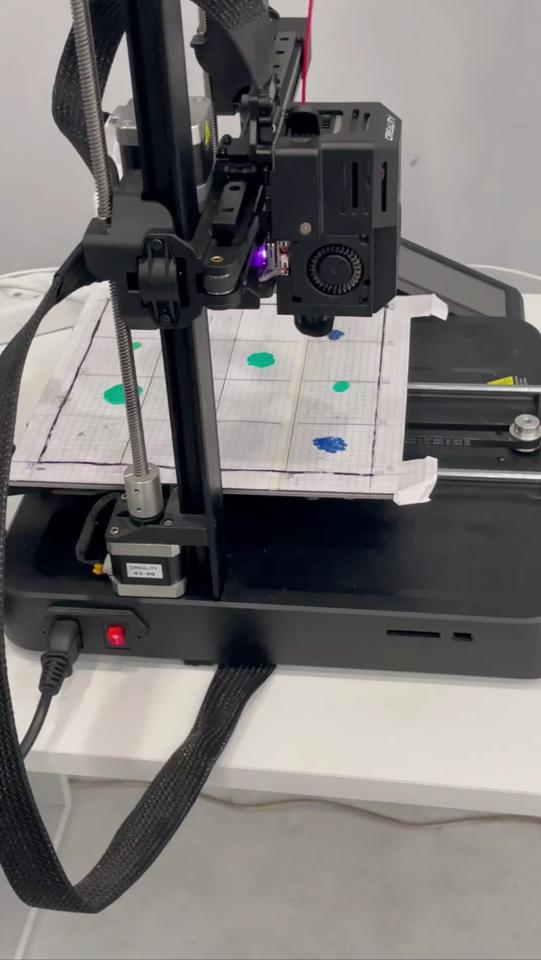
\includegraphics[width=\linewidth,height=80mm,keepaspectratio]{images/hardware-recording.jpg}
\smallcaption{Figure 3. Sampled frame from the supplied \texttt{IMG\_0030.MOV}. Real hardware context.}
\end{minipage}

\subsection{Reproducibility and artifact access}
The repository preserves the four component folders, requirements, setup/check
scripts, offline tests, website screenshots, two recordings and the supplied
10-slide presentation. API keys, SSH passwords, old run histories, camera
calibration and virtual environments are excluded. A fresh network installation
has not been independently verified.

From the repository root, install component environments with
\texttt{python3 scripts/setup.py}. Run the offline Python suites separately with
\texttt{python3 scripts/check.py}. The README documents mock demonstrations and
operator-run real hardware startup.
Scripted demo mode demonstrates the workflow, not live language-model reasoning.

\textbf{Repository:} \href{\repo}{PhotonicsAI-Lab-Cell-Erasing}\\
\textbf{Presentation:} \href{\repo/blob/main/presentation/agentic_cell_erasing_simple.pdf}{Agentic Cell Erasing System (10 slides)}\\
\textbf{Detailed checks:} \href{\repo/blob/main/docs/VALIDATION.md}{Package validation and evidence scope}

\newpage
\section*{(f) Limitations and future applications}
\subsection{Current prototype limits}
Recognition is based on color/image processing and calibrated geometry, not a
trained biological-cell or PCB-defect model. Lighting, occlusion, board movement
and calibration affect measurements. Software tests do not quantify physical
accuracy, removal rate or repeatability. A completed path does not prove that
contact occurred or that ink was erased.

Live language interpretation and visual assessment depend on Groq availability.
Minute/day quotas were encountered during development; the UI now exposes quota
details and Retry-After when supplied. Follow-up references and complex commands
remain bounded by the supported schema. The product is a supervised local lab
prototype, not a general autonomous robot.

\subsection{A reusable platform beyond cell erasing}
The main transferable contribution is the interaction loop: interpret a request,
locate a target, calculate geometry, propose a bounded action, obtain operator
approval, execute and inspect the result. Colored-mark erasing is the first
application used to explore that loop. The following are proposed development
directions, not demonstrated capabilities of the submitted system.

\begin{tabularx}{\linewidth}{@{}>{\raggedright\arraybackslash}p{32mm}Y Y@{}}
\toprule
\textbf{Direction} & \textbf{Possible extension} & \textbf{Required development}\\\midrule
Biomedical laboratories & Select a specimen region; position a camera or measurement probe under operator supervision. & Microscopy-specific recognition, finer positioning, sample-compatible tooling and application-specific validation. No clinical use is demonstrated.\\
PCB inspection and repair support & Locate a component or suspected defect; position a probe or assist a local cleaning operation. & PCB-specific perception, tool calibration, electrical precautions and force/temperature control where relevant. Actual board repair is not demonstrated.\\
Industrial inspection & Measure, mark or locally process a selected surface region. & Material-specific sensing and tooling, defined tolerances and validated before/after criteria.\\
Education and research & Supervised experiments and extensible instrument workflows. & New MCP adapters, repeatable procedures and structured experiment records.\\
\bottomrule
\end{tabularx}

\subsection{Practical next steps}
\begin{enumerate}
\item Measure targeting error and repeatability against independently measured
board coordinates under varied lighting and camera placement.
\item Improve the end effector, establish contact/force feedback and evaluate
removal with controlled before/after trials and predefined acceptance criteria.
\item Reduce model-call overhead and improve quota-aware waiting for interpretation;
retain the prohibition on automatically retrying uncertain physical motion.
\item Adapt perception and tooling to one new domain, then validate that specific
application before expanding the claims.
\end{enumerate}

The prototype demonstrates how a hardware interface can become a conversational,
measured and operator-controlled product. Its broader value is the extensible
architecture; reliable task-specific physical performance is the next milestone.
\end{document}
